% style/preamble throws error, hence preamble4tex is kept here
\documentclass[11pt,compress,t,notes=noshow, xcolor=table]{beamer}
\usepackage[]{graphicx}\usepackage[]{color}
% maxwidth is the original width if it is less than linewidth
% otherwise use linewidth (to make sure the graphics do not exceed the margin)
\makeatletter
\def\maxwidth{ %
  \ifdim\Gin@nat@width>\linewidth
    \linewidth
  \else
    \Gin@nat@width
  \fi
}
\makeatother

\definecolor{fgcolor}{rgb}{0.345, 0.345, 0.345}
\newcommand{\hlnum}[1]{\textcolor[rgb]{0.686,0.059,0.569}{#1}}%
\newcommand{\hlstr}[1]{\textcolor[rgb]{0.192,0.494,0.8}{#1}}%
\newcommand{\hlcom}[1]{\textcolor[rgb]{0.678,0.584,0.686}{\textit{#1}}}%
\newcommand{\hlopt}[1]{\textcolor[rgb]{0,0,0}{#1}}%
\newcommand{\hlstd}[1]{\textcolor[rgb]{0.345,0.345,0.345}{#1}}%
\newcommand{\hlkwa}[1]{\textcolor[rgb]{0.161,0.373,0.58}{\textbf{#1}}}%
\newcommand{\hlkwb}[1]{\textcolor[rgb]{0.69,0.353,0.396}{#1}}%
\newcommand{\hlkwc}[1]{\textcolor[rgb]{0.333,0.667,0.333}{#1}}%
\newcommand{\hlkwd}[1]{\textcolor[rgb]{0.737,0.353,0.396}{\textbf{#1}}}%
\let\hlipl\hlkwb

\usepackage{framed}
\makeatletter
\newenvironment{kframe}{%
 \def\at@end@of@kframe{}%
 \ifinner\ifhmode%
  \def\at@end@of@kframe{\end{minipage}}%
  \begin{minipage}{\columnwidth}%
 \fi\fi%
 \def\FrameCommand##1{\hskip\@totalleftmargin \hskip-\fboxsep
 \colorbox{shadecolor}{##1}\hskip-\fboxsep
     % There is no \\@totalrightmargin, so:
     \hskip-\linewidth \hskip-\@totalleftmargin \hskip\columnwidth}%
 \MakeFramed {\advance\hsize-\width
   \@totalleftmargin\z@ \linewidth\hsize
   \@setminipage}}%
 {\par\unskip\endMakeFramed%
 \at@end@of@kframe}
\makeatother

\definecolor{shadecolor}{rgb}{.97, .97, .97}
\definecolor{messagecolor}{rgb}{0, 0, 0}
\definecolor{warningcolor}{rgb}{1, 0, 1}
\definecolor{errorcolor}{rgb}{1, 0, 0}
\newenvironment{knitrout}{}{} % an empty environment to be redefined in TeX

\usepackage{alltt}
\newcommand{\SweaveOpts}[1]{}  % do not interfere with LaTeX
\newcommand{\SweaveInput}[1]{} % because they are not real TeX commands
\newcommand{\Sexpr}[1]{}       % will only be parsed by R
\newcommand{\xmark}{\ding{55}}%


\usepackage[english]{babel}
\usepackage[utf8]{inputenc}

\usepackage{dsfont}
\usepackage{verbatim}
\usepackage{amsmath}
\usepackage{amsfonts}
\usepackage{amssymb}
\usepackage{bm}
\usepackage{csquotes}
\usepackage{multirow}
\usepackage{longtable}
\usepackage{booktabs}
\usepackage{enumerate}
\usepackage[absolute,overlay]{textpos}
\usepackage{psfrag}
\usepackage{algorithm}
\usepackage{algpseudocode}
\usepackage{eqnarray}
\usepackage{arydshln}
\usepackage{tabularx}
\usepackage{placeins}
\usepackage{tikz}
\usepackage{setspace}
\usepackage{colortbl}
\usepackage{mathtools}
\usepackage{wrapfig}
\usepackage{bm}
\usepackage{amsmath}
\usepackage{pifont}
\usepackage{xcolor} %colored math symbols

\usetikzlibrary{shapes,arrows,automata,positioning,calc,chains,trees, shadows}
\tikzset{
  %Define standard arrow tip
  >=stealth',
  %Define style for boxes
  punkt/.style={
    rectangle,
    rounded corners,
    draw=black, very thick,
    text width=6.5em,
    minimum height=2em,
    text centered},
  % Define arrow style
  pil/.style={
    ->,
    thick,
    shorten <=2pt,
    shorten >=2pt,}
}

\usepackage{subfig}

% Defines macros and environments
\usepackage{../../style/lmu-lecture}


\let\code=\texttt
\let\proglang=\textsf

\setkeys{Gin}{width=0.9\textwidth}

\setbeamertemplate{frametitle}{\expandafter\uppercase\expandafter\insertframetitle}

\usepackage{bbm}
% basic latex stuff
\newcommand{\pkg}[1]{{\fontseries{b}\selectfont #1}} %fontstyle for R packages
\newcommand{\lz}{\vspace{0.5cm}} %vertical space
\newcommand{\dlz}{\vspace{1cm}} %double vertical space
\newcommand{\oneliner}[1] % Oneliner for important statements
{\begin{block}{}\begin{center}\begin{Large}#1\end{Large}\end{center}\end{block}}


%new environments
\newenvironment{vbframe}  %frame with breaks and verbatim
{
 \begin{frame}[containsverbatim,allowframebreaks]
}
{
\end{frame}
}

\newenvironment{vframe}  %frame with verbatim without breaks (to avoid numbering one slided frames)
{
 \begin{frame}[containsverbatim]
}
{
\end{frame}
}

\newenvironment{blocki}[1]   % itemize block
{
 \begin{block}{#1}\begin{itemize}
}
{
\end{itemize}\end{block}
}

\newenvironment{fragileframe}[2]{  %fragile frame with framebreaks
\begin{frame}[allowframebreaks, fragile, environment = fragileframe]
\frametitle{#1}
#2}
{\end{frame}}


\newcommand{\myframe}[2]{  %short for frame with framebreaks
\begin{frame}[allowframebreaks]
\frametitle{#1}
#2
\end{frame}}

\newcommand{\remark}[1]{
  \textbf{Remark:} #1
}


\newenvironment{deleteframe}
{
\begingroup
\usebackgroundtemplate{
\includegraphics[width=\paperwidth,height=\paperheight]{../style/color/red.png}}
 \begin{frame}
}
{
\end{frame}
\endgroup
}
\newenvironment{simplifyframe}
{
\begingroup
\usebackgroundtemplate{
\includegraphics[width=\paperwidth,height=\paperheight]{../style/color/yellow.png}}
 \begin{frame}
}
{
\end{frame}
\endgroup
}\newenvironment{draftframe}
{
\begingroup
\usebackgroundtemplate{
\includegraphics[width=\paperwidth,height=\paperheight]{../style/color/green.jpg}}
 \begin{frame}
}
{
\end{frame}
\endgroup
}
% https://tex.stackexchange.com/a/261480: textcolor that works in mathmode
\makeatletter
\renewcommand*{\@textcolor}[3]{%
  \protect\leavevmode
  \begingroup
    \color#1{#2}#3%
  \endgroup
}
\makeatother


\input{../../latex-math/basic-math}
\input{../../latex-math/basic-ml}
\input{../../latex-math/ml-nn}

\newcommand{\titlefigure}{figure/backprop_gg_new.png}
\newcommand{\learninggoals}{
  \item Forward and backward passes
  \item Chain rule
  \item Details of backprop
}

\title{Deep Learning}
\date{}

\begin{document}

\lecturechapter{Basic Backpropagation 1}
\lecture{I2DL}
%%%%%%%%%%%%%%%%%%%%%%%%%%%%%%%%%%%%%%%%%%%%%%%%%%%%%%%%%%%%%%%%%%

\begin{frame}{Backpropagation: Basic Idea}
We would like to run ERM by GD on: $$ \risket = \frac{1}{n} \sumin \Lxyit$$ 
% where $\thetab$ are the weights (and biases) of the network. 

Backprop training of NNs runs in 2 alternating steps, for one $\xv$:
\begin{enumerate}
\item \textbf{Forward pass:} Inputs flow through model to outputs. 
    We then compute the observation loss. We covered that.
\item \textbf{Backward pass:} Loss flows backwards to update weights so error is reduced,
    as in GD.
\end{enumerate}
\lz
We will see: This is simply (S)GD in disguise, cleverly using the chain rule, so we can reuse
a lot of intermediate results.
\end{frame}
%%%%%%%%%%%%%%%%%%%%%%%%%%%%%%%%%%%%%%%%%%%%%%%%%%%%%%%%%%%%%%%%%%

% \begin{vbframe}{Weight update rule}
  % \begin{itemize}
    % \item Backpropagation can then be used to compute the gradient of $\Lxyt$ in an \textbf{extremely} efficient way.
    % \item  In GD, the weight for one $\xv$ with learning rate $\alpha$, is 
      % $$\thetab^{[t+1]} = \thetab^{[t]} - \alpha \cdot \nabla_{\theta}L\left(y, f\left(\xv ~|~ \thetab^{[t]}\right)\right)$$ 
        % \item We will see that, at its core, backpropagation is just a clever implementation of the chain rule. Nothing more!

  % \item We could now sum up these gradients for all $\xi$ from $\Dset$ to compute the gradient over the complete training set, to perform a full GD step. But as we want to arrive at stochastic gradient descent, 
    % we stick for now with updates for a single $\xv$.
  % \end{itemize}
% \end{vbframe}
%%%%%%%%%%%%%%%%%%%%%%%%%%%%%%%%%%%%%%%%%%%%%%%%%%%%%%%%%%%%%%%%%%


\begin{vbframe}{XOR example}
  \begin{itemize}
    % \item Let us recall the XOR example. 
    \item As activations (hidden and outputs) we use the logistic.
    \item We run one FP and BP on $\xv = (1,0)^T$ with $y=1$.
    \item We use L2 loss between 0-1 labels and the predicted probabilities.
        This is a bit uncommon, but computations become simpler.
        % for this instructive example.
    % \item Then we compute the backward pass and apply backpropagation to update the weights.
    % \item Finally we evaluate the model with our updated weights.
  \end{itemize}
  \begin{figure}
    \centering
      \scalebox{0.7}{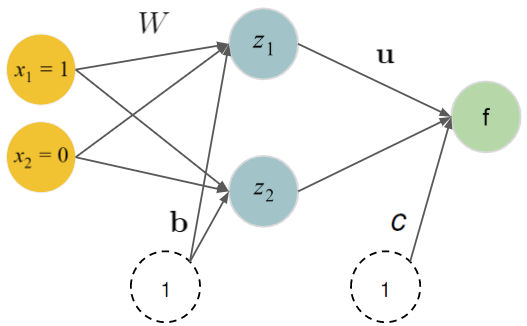
\includegraphics{figure/forwardprop1_new.png}}
      % \caption{A neural network with two neurons in the hidden layer. $W$ and $\biasb$ are the weights and biases of the hidden layer. $\wtu$ and $c$ are the weights and bias of the output layer. Based on the values for the weights (and biases), we will perform one forward and one backward pass.}
  \end{figure}
\begin{footnotesize}
  Note: We will only show rounded decimals. 
\end{footnotesize}
% \framebreak
\end{vbframe} 

\begin{vbframe}{ Forward pass}

\begin{itemize}
\item We will divide the FP into four steps:
\begin{itemize}
\item the inputs of $z_i$: $\bm{{z_{i,in}}}$
\item the activations of $z_i$: $\bm{{z_{i,out}}}$
\item the input of $f$: $\bm{{f_{in}}}$
\item and finally the activation of $f$: $\bm{{f_{out}}}$
\end{itemize}
\begin{figure}
\centering
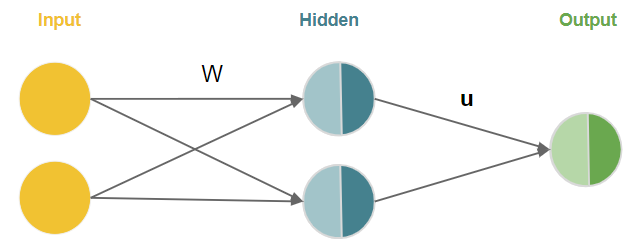
\includegraphics[width=8cm]{figure/xor_rep.png}
\end{figure}
\begin{figure}
\centering
\scalebox{0.5}{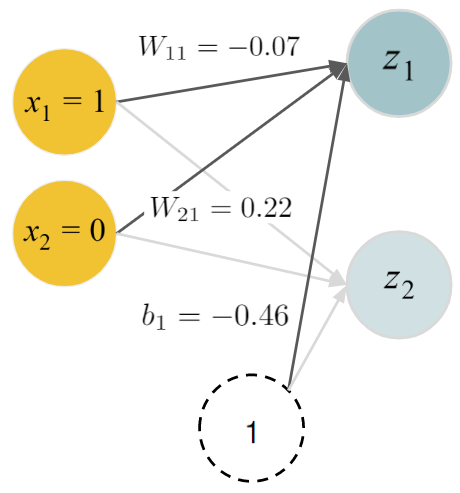
\includegraphics{figure/forwardprop2b_new.png}}
\end{figure}
\begin{footnotesize}
\begin{eqnarray*}
z_{1,in} &=& \Wmat_1^T \xv + b_1 =  1 \cdot (-0.07) + 0 \cdot 0.22 + 1 \cdot (-0.46) = -0.53 \\
z_{1,out} &=& \sigma\left(z_{1,in}\right) = \frac{1}{1+\exp(-(-0.53))} = \num[round-mode=places,round-precision=4]{0.3705169}
\end{eqnarray*}
\end{footnotesize}
\end{itemize}
\framebreak
%%%%%%%%%%%%%%%%%%%%%%%%%%%%%%%%%%%%%%%%%%%%%%%%%%%%%%%%%%%%%%%%%%

  \begin{figure}
    \centering
      \scalebox{0.5}{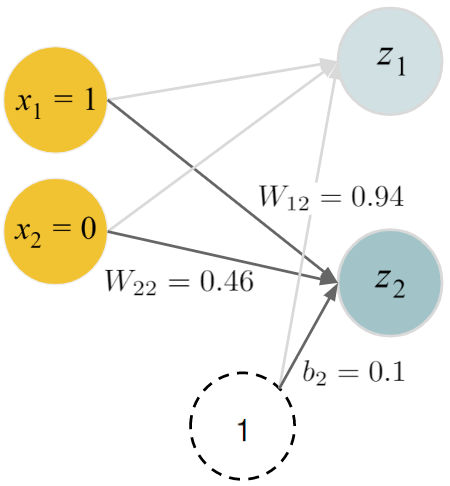
\includegraphics{figure/forwardprop3b_new.png}}
  \end{figure}
\vspace*{-0.5cm}
  \begin{footnotesize}
    \begin{eqnarray*}
    z_{2,in} &=& \Wmat_2^T \xv + b_2 = 1 \cdot 0.94 + 0 \cdot 0.46 + 1 \cdot 0.1 = 1.04 \\
    z_{2,out} &=& \sigma\left(z_{2,in}\right) = \frac{1}{1+\exp(-1.04)} = \num[round-mode=places,round-precision=4]{0.73885}
    \end{eqnarray*}
  \end{footnotesize}
\framebreak
%%%%%%%%%%%%%%%%%%%%%%%%%%%%%%%%%%%%%%%%%%%%%%%%%%%%%%%%%%%%%%%%%%

  \begin{figure}
    \centering
      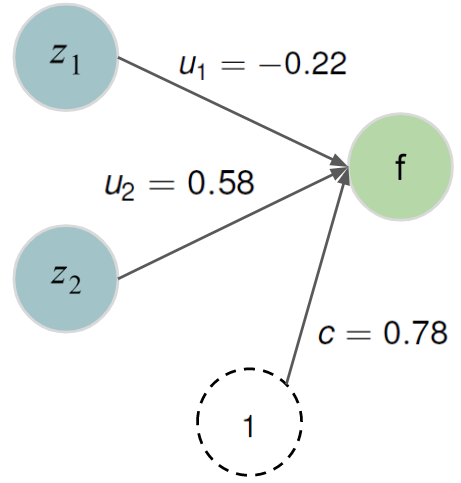
\includegraphics[width=5cm]{figure/forwardprop4b_new.png}
  \end{figure}

\vspace*{-0.5cm}

  \begin{footnotesize}
    \begin{eqnarray*}
    f_{in} &=& \bm{u}^T \bm{z} + c = \num[round-mode=places,round-precision=4]{0.3705169} \cdot (-0.22) + \num[round-mode=places,round-precision=4]{0.73885} \cdot 0.58 + 1 \cdot 0.78 = \num[round-mode=places,round-precision=4]{1.112242} \\
    f_{out} &=& \tau\left(f_{in}\right) = \frac{1}{1+\exp(\num[round-mode=places,round-precision=4]{-1.112242})} = \num[round-mode=places,round-precision=4]{0.7525469}
    \end{eqnarray*}
  \end{footnotesize}
\framebreak
%%%%%%%%%%%%%%%%%%%%%%%%%%%%%%%%%%%%%%%%%%%%%%%%%%%%%%%%%%%%%%%%%%

  \begin{itemize}
    \item The FP predicted $f_{out} = 0.7525$
    \item Now, we compare the prediction $f_{out} = 0.7525$ and the true label $y = 1$ using the L2-loss: 
      \begin{eqnarray*}
        \Lxy &=& \frac{1}{2}(y - \fxit)^2 = \frac{1}{2}\left(y - f_{out}\right)^{2} \\
                  &=& \frac{1}{2}\left(1 - \num[round-mode=places,round-precision=4]{0.7525469}\right)^2 = \num[round-mode=places,round-precision=4]{0.03061652}
      \end{eqnarray*}
    \item The calculation of the gradient is performed backwards (starting from the output layer), so that results can be reused. 
\end{itemize}
\end{vbframe}
%%%%%%%%%%%%%%%%%%%%%%%%%%%%%%%%%%%%%%%%%%%%%%%%%%%%%%%%%%%%%%%%%%

\begin{vbframe}{Backward pass}
% \begin{itemize}
   The main ingredients of the backward pass are: 
    \begin{itemize}
      \item to reuse the results of the forward pass \\ (here:  ${z_{i, in}, z_{i, out}, f_{in},f_{out}}$)
      \item reuse the \textcolor{violet}{intermediate results} from the chain rule 
      \item the derivative of the activations and some affine functions
    \end{itemize}
    % \item This is demonstrated by continuing the example above.
      % \end{itemize}
\framebreak
%%%%%%%%%%%%%%%%%%%%%%%%%%%%%%%%%%%%%%%%%%%%%%%%%%%%%%%%%%%%%%%%%%

  \begin{itemize}
    \item Let's start to update $u_1$. We recursively apply the chain rule: $$\frac{\partial \Lxy}{\partial u_1} = \frac{\partial \Lxy}{\partial f_{out}} \cdot \frac{\partial f_{out}}{\partial f_{in}} \cdot \frac{\partial f_{in}}{\partial u_1}$$
  \end{itemize}
  \begin{figure}
    \centering
      \scalebox{0.54}{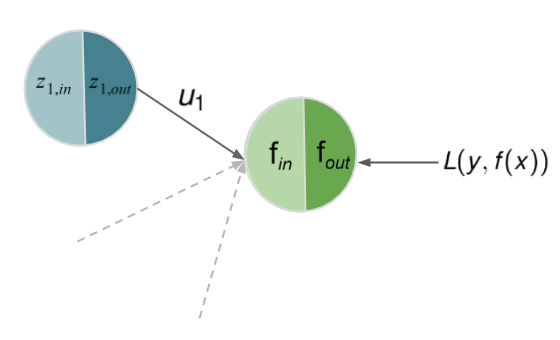
\includegraphics{figure/backprop1_new.png}}
      \caption{\footnotesize{Snippet from our NN, with backward path for $u_1$.}}
  \end{figure}
\framebreak
%%%%%%%%%%%%%%%%%%%%%%%%%%%%%%%%%%%%%%%%%%%%%%%%%%%%%%%%%%%%%%%%%%

  \begin{itemize}
    \item 1st step: The derivative of L2 is easy; we know ${f_{out}}$ from FP.
  \end{itemize}
    \begin{eqnarray*}
      \textcolor{violet}{\frac{\partial \Lxy}{\partial f_{out}}} &=& \frac{d}{\partial f_{out}} \frac{1}{2}(y - f_{out})^2 = -\underbrace{(y - {f_{out}})}_{\hat{=} \text{residual}} \\
       &=& -(1 - \num[round-mode=places,round-precision=4]{0.7525469}) = \num[round-mode=places,round-precision=4]{-0.2474531}
    \end{eqnarray*}
    \begin{figure}
      \centering
        \scalebox{0.6}{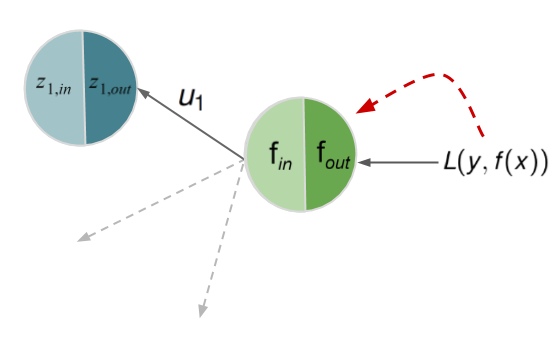
\includegraphics{figure/backprop1_b_new.png}}
        % \caption{The first term of our chain rule $\frac{\partial \Lxy}{\partial f_{out}}$}
    \end{figure}
\framebreak
%%%%%%%%%%%%%%%%%%%%%%%%%%%%%%%%%%%%%%%%%%%%%%%%%%%%%%%%%%%%%%%%%%

  \begin{itemize}
    \item 2nd step. $f_{out} = \sigma(f_{in})$, use rule for $\sigma'$, use ${f_{in}}$ from FP.
  \end{itemize}
    \begin{eqnarray*}
      \textcolor{violet}{\frac{\partial f_{out}}{\partial f_{in}}}  &=& \sigma({f_{in}})\cdot(1-\sigma({f_{in}})) \\
      &=& \num[round-mode=places,round-precision=4]{0.7525469} \cdot (1 - \num[round-mode=places,round-precision=4]{0.7525469}) = \num[round-mode=places,round-precision=4]{0.1862201}
    \end{eqnarray*}
      \vspace{-0.5cm}
    \begin{figure}
      \centering
        \scalebox{0.6}{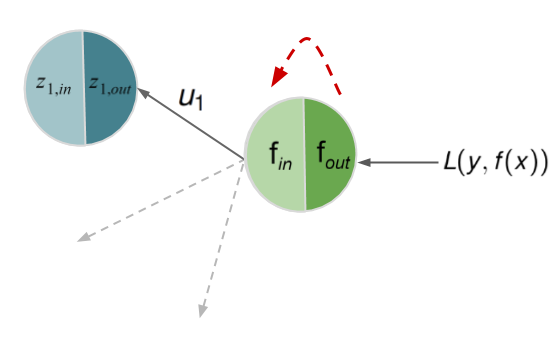
\includegraphics{figure/backprop1_c_new.png}}
        % \caption{The second term of our chain rule $\frac{\partial f_{out}}{\partial f_{in}}$}
    \end{figure}
\framebreak
%%%%%%%%%%%%%%%%%%%%%%%%%%%%%%%%%%%%%%%%%%%%%%%%%%%%%%%%%%%%%%%%%%

  \begin{itemize}
    \item 3rd step. Derivative of the linear input is easy; use ${z_{1, out}}$ from FP.
  \end{itemize}
    \begin{eqnarray*}
      \textcolor{violet}{\frac{\partial f_{in}}{\partial u_1}} = \frac{\partial (u_1 \cdot z_{1,out} + u_2 \cdot z_{2,out} + c \cdot 1)}{\partial u_1} = {z_{1, out}} = \num[round-mode=places,round-precision=4]{0.3705169}
    \end{eqnarray*}
    \begin{figure}
      \centering
        \scalebox{0.6}{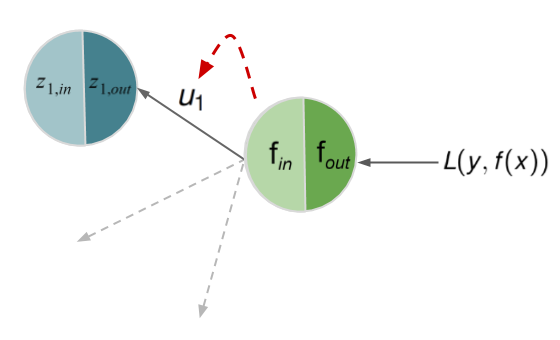
\includegraphics{figure/backprop1_d_new.png}}
        % \caption{The third term of our chain rule $\frac{\partial f_{in}}{\partial u_1}$}
    \end{figure}
\framebreak
%%%%%%%%%%%%%%%%%%%%%%%%%%%%%%%%%%%%%%%%%%%%%%%%%%%%%%%%%%%%%%%%%%

  \begin{itemize}
    \item Plug it together:
  \begin{eqnarray*}
    \textcolor{violet}{\frac{\partial \Lxy}{\partial u_1}} &=& \textcolor{violet}{\frac{\partial \Lxy}{\partial f_{out}}} \cdot \textcolor{violet}{\frac{\partial f_{out}}{\partial f_{in}}} \cdot \textcolor{violet}{\frac{\partial f_{in}}{\partial u_1}} \\
                                        &=& \num[round-mode=places,round-precision=4]{-0.2474531} \cdot \num[round-mode=places,round-precision=4]{0.1862201} \cdot \num[round-mode=places,round-precision=4]{0.3705169} = \num[round-mode=places,round-precision=4]{-0.01707369}
  \end{eqnarray*}
    \begin{figure}
      \centering
        \scalebox{0.4}{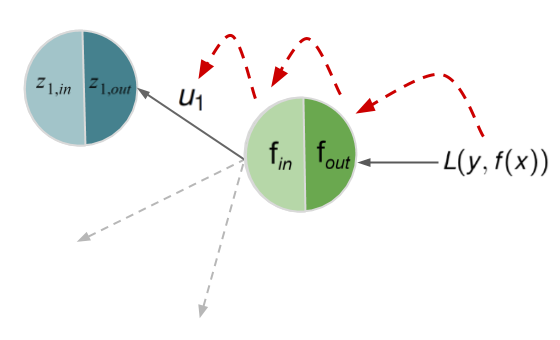
\includegraphics{figure/backprop1_e_new.png}}
        % \caption{All three terms of our chain rule $\frac{\partial \Lxy}{\partial u_1} = \frac{\partial \Lxy}{\partial f_{out}} \cdot \frac{\partial f_{out}}{\partial f_{in}} \cdot \frac{\partial f_{in}}{\partial u_1}$}
    \end{figure}
% \framebreak
%%%%%%%%%%%%%%%%%%%%%%%%%%%%%%%%%%%%%%%%%%%%%%%%%%%%%%%%%%%%%%%%%%

  % \begin{itemize}
\item  With LR $\alpha = 0.5$:
  % \end{itemize}
    \begin{eqnarray*}
      u_1^{[new]} &=& u_1^{[old]} - \alpha \cdot \textcolor{violet}{\frac{\partial \Lxy}{\partial u_1}} \\
                &=& -0.22 - 0.5 \cdot (\num[round-mode=places,round-precision=4]{-0.01707369}) = \num[round-mode=places,round-precision=4]{-0.2114632}
    \end{eqnarray*}
  \end{itemize}
\framebreak
%%%%%%%%%%%%%%%%%%%%%%%%%%%%%%%%%%%%%%%%%%%%%%%%%%%%%%%%%%%%%%%%%%

  \begin{itemize}
    \item Now for $W_{11}$: $$\frac{\partial \Lxy}{\partial W_{11}} = \textcolor{violet}{\frac{\partial \Lxy}{\partial f_{out}}} \cdot \textcolor{violet}{\frac{\partial f_{out}}{\partial f_{in}}} \cdot \frac{\partial f_{in}}{\partial z_{1,out}} \cdot \frac{\partial z_{1,out}}{\partial z_{1,in}} \cdot \frac{\partial z_{1,in}}{\partial W_{11}}$$
  \end{itemize}
  % \begin{figure}
    % \centering
      % \scalebox{0.70}{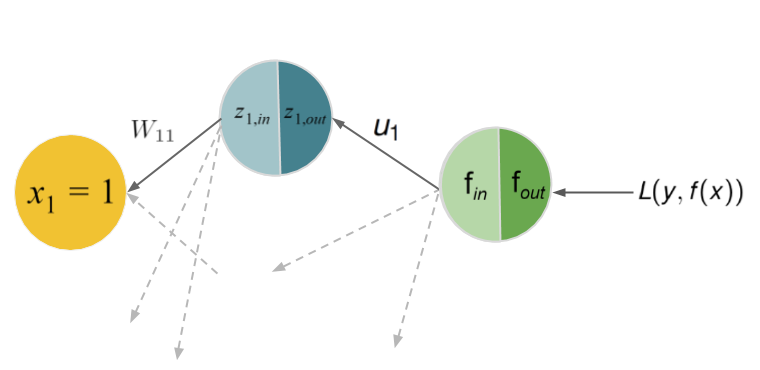
\includegraphics{figure/backprop2_new.png}}
      % \caption{Snippet from our neural network showing the backward path to compute the gradient with respect to weight $W_{11}$.}
  % \end{figure}
% \framebreak
%%%%%%%%%%%%%%%%%%%%%%%%%%%%%%%%%%%%%%%%%%%%%%%%%%%%%%%%%%%%%%%%%%

  \begin{itemize}
    \item We know $\textcolor{violet}{\frac{\partial \Lxy}{\partial f_{out}}}$ and $\textcolor{violet}{\frac{\partial f_{out}}{\partial f_{in}}}$ from BP for $u_1$.
  \begin{figure}
    \centering
      \scalebox{0.7}{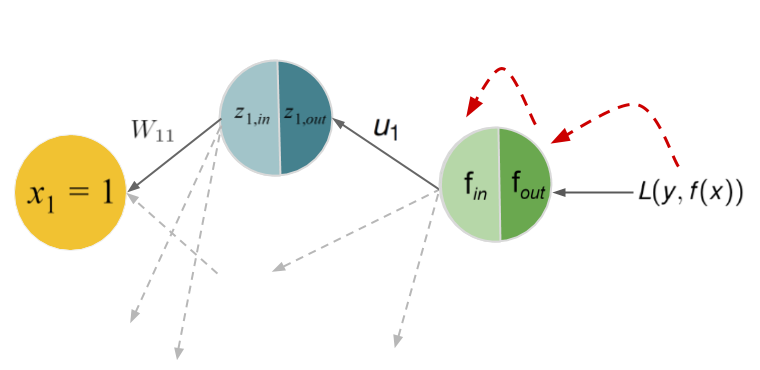
\includegraphics{figure/backprop2_bc_new.png}}
      % \caption{The first and second term of our chain rule $\frac{\partial \Lxy}{\partial f_{out}}$ and $\frac{\partial f_{out}}{\partial f_{in}}$}
  \end{figure}
\framebreak
%%%%%%%%%%%%%%%%%%%%%%%%%%%%%%%%%%%%%%%%%%%%%%%%%%%%%%%%%%%%%%%%%%

    \item $f_{in} = u_1 \cdot z_{1,out} + u_2 \cdot z_{2,out} + c \cdot 1$ is linear, easy and we know $u_1$ :
  \end{itemize}
  \begin{eqnarray*}
    \textcolor{violet}{\frac{\partial f_{in}}{\partial z_{1,out}}} = u_1 = -0.22
  \end{eqnarray*}
  \begin{figure}
    \centering
      \scalebox{0.7}{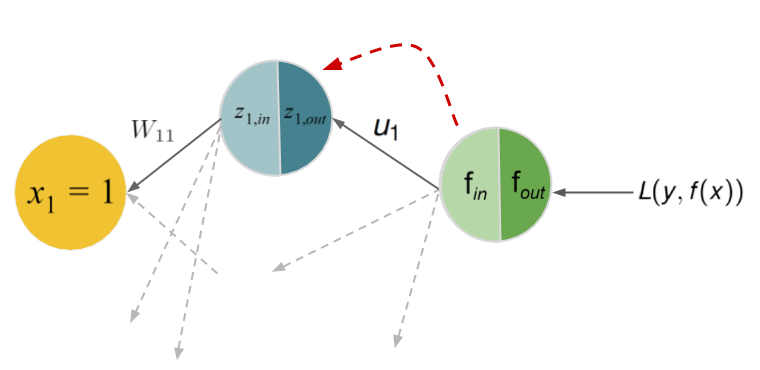
\includegraphics{figure/backprop2_d_new.png}}
      % \caption{The third term of our chain rule $\frac{\partial f_{in}}{\partial z_{1,out}}$}
  \end{figure}
\framebreak
%%%%%%%%%%%%%%%%%%%%%%%%%%%%%%%%%%%%%%%%%%%%%%%%%%%%%%%%%%%%%%%%%%

  \begin{itemize}
    \item Next. Use rule for $\sigma'$ and FP results:
  \end{itemize}
  \begin{eqnarray*}
    \textcolor{violet}{\frac{\partial z_{1,out}}{\partial z_{1,in}}}  &=& \sigma({z_{1,in}}) \cdot (1-\sigma({z_{1,in}})) \\&=&  \num[round-mode=places,round-precision=4]{0.3705169} \cdot (1 - \num[round-mode=places,round-precision=4]{0.3705169}) = \num[round-mode=places,round-precision=4]{0.2332341}
  \end{eqnarray*}
  \begin{figure}
    \centering
      \scalebox{0.7}{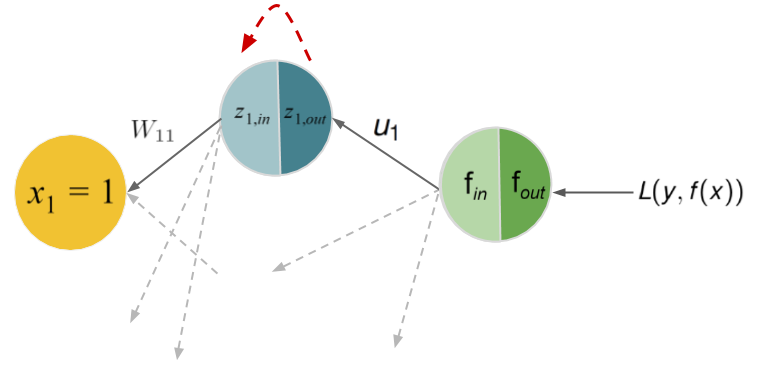
\includegraphics{figure/backprop2_e_new.png}}
      % \caption{The fourth term of our chain rule $\frac{\partial z_{1,out}}{\partial z_{1,in}}$}
  \end{figure}
\framebreak
%%%%%%%%%%%%%%%%%%%%%%%%%%%%%%%%%%%%%%%%%%%%%%%%%%%%%%%%%%%%%%%%%%

  \begin{itemize}
    \item $z_{1,in} = x_1 \cdot W_{11} + x_2 \cdot W_{21} + b_1 \cdot 1$ is linear
        and depends on inputs:
  \end{itemize}
  \begin{eqnarray*}
    \textcolor{violet}{\frac{\partial z_{1,in}}{\partial W_{11}}} = x_1 = 1
  \end{eqnarray*}
  \begin{figure}
    \centering
      \scalebox{0.65}{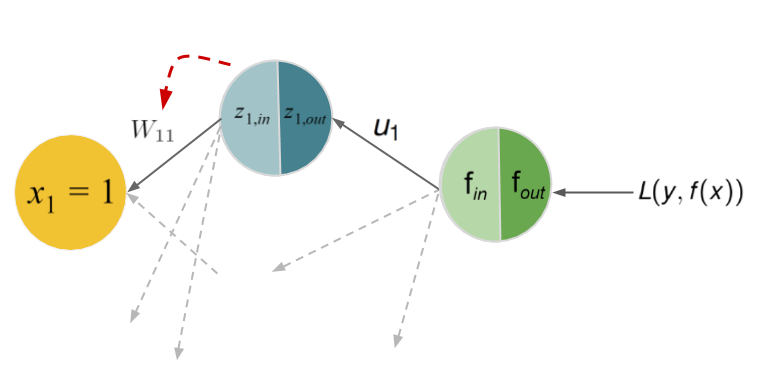
\includegraphics{figure/backprop2_f_new.png}}
      % \caption{The fifth term of our chain rule $\frac{\partial z_{1,in}}{\partial W_{11}}$}
  \end{figure}
\framebreak
%%%%%%%%%%%%%%%%%%%%%%%%%%%%%%%%%%%%%%%%%%%%%%%%%%%%%%%%%%%%%%%%%%

  \begin{itemize}
    \item Plugging together: 
      \begin{eqnarray*}
         \textcolor{violet}{\frac{\partial \Lxy}{\partial W_{11}}} &=& 
         \textcolor{violet}{\frac{\partial \Lxy}{\partial f_{out}}} \cdot  \textcolor{violet}{\frac{\partial f_{out}}{\partial f_{in}}} \cdot  \textcolor{violet}{\frac{\partial f_{in}}{\partial z_{1,out}}} \cdot  \textcolor{violet}{\frac{\partial z_{1,out}}{\partial z_{1,in}}} \cdot  \textcolor{violet}{\frac{\partial z_{1,in}}{\partial W_{11}}} 
        \\ &=& (\num[round-mode=places,round-precision=4]{-0.2474531}) \cdot \num[round-mode=places,round-precision=4]{0.1862201} \cdot (-0.22) \cdot \num[round-mode=places,round-precision=4]{0.2332341} \cdot 1 
        \\ &=& \num[round-mode=places,round-precision=4]{0.0023645}
      \end{eqnarray*}
  \begin{figure}
    \centering
      \scalebox{0.5}{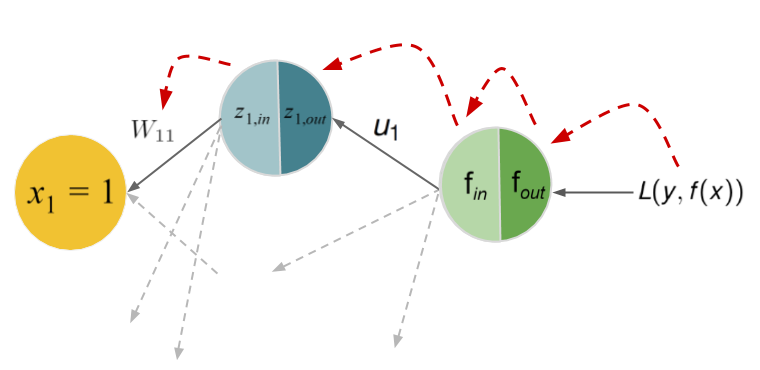
\includegraphics{figure/backprop2_g_new.png}}
      % \caption{All five terms of our chain rule}
  \end{figure}
% \framebreak
%%%%%%%%%%%%%%%%%%%%%%%%%%%%%%%%%%%%%%%%%%%%%%%%%%%%%%%%%%%%%%%%%%

    \item Full SGD update: 
    \begin{eqnarray*}
      W_{11}^{[new]}  &=& W_{11}^{[old]} - \alpha \cdot  \textcolor{violet}{\frac{\partial \Lxy}{\partial W_{11}}} \\
                  &=& -0.07 - 0.5 \cdot \num[round-mode=places,round-precision=4]{0.0023645} = \num[round-mode=places,round-precision=4]{-0.0711823}
    \end{eqnarray*}
  \end{itemize}
\end{vbframe}

\begin{vbframe}{Result}
  \begin{itemize}
    \item We can do this for all weights:
  \end{itemize}
  \begin{eqnarray*}
    W = \begin{pmatrix}
    \num[round-mode=places,round-precision=4]{-0.0711823} & \num[round-mode=places,round-precision=4]{0.9425785} \\
    0.22 & 0.46
    \end{pmatrix},
    b = \begin{pmatrix}
    \num[round-mode=places,round-precision=4]{-0.4611822} \\
    \num[round-mode=places,round-precision=4]{0.1025782}
    \end{pmatrix},
  \end{eqnarray*}
  \begin{eqnarray*}
    u = \begin{pmatrix}
    \num[round-mode=places,round-precision=4]{-0.2114632} \\
    \num[round-mode=places,round-precision=4]{0.5970234}
    \end{pmatrix}
    \text{and} \ c = \num[round-mode=places,round-precision=4]{0.8030404}\text{.}
  \end{eqnarray*}
% \framebreak  
%%%%%%%%%%%%%%%%%%%%%%%%%%%%%%%%%%%%%%%%%%%%%%%%%%%%%%%%%%%%%%%%%%

  \begin{itemize}
    \item Yields $f(\xv ~|~\thetab^{[new]}) = \num[round-mode=places,round-precision=4]{0.7614865}$ and loss 
        $\frac{1}{2}(1 - \num[round-mode=places,round-precision=4]{0.7614865})^2 = \num[round-mode=places,round-precision=4]{0.02844434}.$
        % $\Lxy = \frac{1}{2}(1 - \num[round-mode=places,round-precision=4]{0.7614865})^2 = \num[round-mode=places,round-precision=4]{0.02844434}.$$
    \item Before, we had $f(\xv ~|~\thetab^{[old]}) = \num[round-mode=places,round-precision=4]{0.7525469}$ and higher loss $\num[round-mode=places,round-precision=4]{0.03061652}$.

  \end{itemize}
\lz
 Now rinse and repeat. This was one training iter, we do thousands.
\end{vbframe}
%%%%%%%%%%%%%%%%%%%%%%%%%%%%%%%%%%%%%%%%%%%%%%%%%%%%%%%%%%%%%%%%%%

% \begin{frame} { Summary}
%   \begin{itemize}
%     \item Our goal was to minimize the true/expected risk $$\riskt = \E_{(\xv, y)\sim \Pxy} \left[\Lxyt\right]$$
%     with respect to the true underlying distribution $\Pxy$.
%     \item Because we do not know $\Pxy$, we decided to minimize the empirical risk $$\risket = \frac{1}{n} \sumin \Lxyit$$ w.r.t. the training set and hope for the best.
%     \item However, even this is not possible because there is no way to analytically find a global minimum for deep neural networks.
%     \item Therefore, we decided to use gradient descent to iteratively find a local minimum of the (typically) non-convex loss function.
%   \end{itemize}
% \end{frame}
%%%%%%%%%%%%%%%%%%%%%%%%%%%%%%%%%%%%%%%%%%%%%%%%%%%%%%%%%%%%%%%%%%

% \begin{frame} { Summary}
  % \begin{itemize}
      % \item To perform gradient descent, we want to compute the gradient of the loss function $\risket$ with respect to \textbf{all} the weights and biases in the network.
      % \item Therefore, the number of components in the gradient is the total number of weights and biases in the network.
      % \item To compute each component of the gradient, we apply the chain rule to the relevant portion of the computational graph.
      % \item In software, a vectorized version of the chain rule is used to compute the derivatives w.r.t. multiple weights simultaneously.
      % \item Loosely speaking, each term in the gradient represents the extent to which the corresponding weight is responsible for the loss. In other words, it is a way to assign "blame" to each weight.
  % \end{itemize}
% \end{frame}
%%%%%%%%%%%%%%%%%%%%%%%%%%%%%%%%%%%%%%%%%%%%%%%%%%%%%%%%%%%%%%%%%%

% \begin{vbframe} { Summary}

  % \begin{itemize}
    % \item Gradient descent can be implemented efficiently: 
    % \begin{itemize}
      % \item We can store and reuse results of the forward pass
      % \item We reuse intermediate results from the chain rule during the BP.  
      % \item We know how derivates of activation functions and affine functions look like
    % \end{itemize}
    % For example, to compute the derivative of the sigmoid activation at $z_{1,out}$, we \enquote{stored} the derivative of the sigmoid function $\frac{\partial z_{1,out}}{\partial z_{1,in}} = \sigma(z_{1,in})(1-\sigma(z_{1,in}))$ and plugged in $\sigma(z_{1,in}) = \num[round-mode=places,round-precision=4]{0.3705169}$, which was known from the forward pass.
% \end{itemize}
% \framebreak  
%%%%%%%%%%%%%%%%%%%%%%%%%%%%%%%%%%%%%%%%%%%%%%%%%%%%%%%%%%%%%%%%%%

  % \begin{itemize}
  % \item In our example, we updated w.r.t. a single training example but typically, we feed subsets of the training set (minibatch GD).
    % \item The term \enquote{backpropagation} refers to the fact that the computation of the gradient using the chain rule is performed backwards (that is, starting at the output layer and finishing at the first hidden layer). 
      % A \textbf{forward} computation using the chain rule also results in the same gradient but can be computationally expensive (see http://colah.github.io/posts/2015-08-Backprop/).
 % \end{itemize}
% \end{frame} 
%%%%%%%%%%%%%%%%%%%%%%%%%%%%%%%%%%%%%%%%%%%%%%%%%%%%%%%%%%%%%%%%%%

% \begin{frame} { Summary}
%   \begin{itemize}
%     \item After computing the gradient (using backpropagation), we subtract the gradient (scaled by the learning-rate $\alpha$) from the current set of weights (and biases) which results in a new set of weights (and biases).
%     \item The empirical loss for this new set of weights is now lower ("walking down the hill").
%     \item Next, we once again compute the forward pass for this new set of weights and store the activations.
%     \item Then, we compute the gradient of the empirical loss using backpropagation and take another step down the hill.
%     \item Rinse and repeat (until the loss stops decreasing substantially). 
%       However, training until convergence often results in overfitting (use early stopping).
%   \end{itemize}
% \end{frame}
%%%%%%%%%%%%%%%%%%%%%%%%%%%%%%%%%%%%%%%%%%%%%%%%%%%%%%%%%%%%%%%%%%

\endlecture
\end{document}
